% !BIB TS-program = biber
% !BIB program = biber
\documentclass{sgreport}

% PACKAGES
\usepackage[T1]{fontenc}
\usepackage[english]{babel}
\usepackage{lipsum}
\usepackage[dvipsnames,table]{xcolor}
\usepackage{gitinfo2}
\usepackage{hyperref}
\usepackage{soul}
\usepackage{enumerate}
\usepackage[toc, nosuper]{glossaries}
\usepackage{csquotes}
\usepackage{graphicx}
\usepackage{booktabs}
\usepackage{tabu}
\usepackage{longtable}
\usepackage{fdsymbol}
\usepackage{listings}
\usepackage{color}
\usepackage[
backend=biber,
style=numeric-comp,
sorting=ynt
]{biblatex}

% PARAMS
\graphicspath{{images/}}
\setlongtables{}
\definecolor{lightgray}{gray}{0.8}
\definecolor{aliceblue}{rgb}{0.94, 0.97, 1.0}
\definecolor{beaublue}{rgb}{0.74, 0.83, 0.9}

% BIBLIO AND GLOSSARY
\addbibresource{bibliography/p1_bib.bib}
\makeglossaries{}
%------------ GLOSSARY--------------
\newglossaryentry{latex}
{
    name=\LaTeX,
    description={Is a mark up language specially suited for scientific documents}
}
\newglossaryentry{tex}
{
    name=\TeX,
    description={Is a typesetting system developed by Donald Knuth}
}
\newglossaryentry{microsoft_word}
{
    name={Microsoft Word},
    description={Is a word processor created and developed by Microsoft}
}
\newglossaryentry{google_docs}
{
    name={Google Docs},
    description={Is an online word processor created and developed by Google}
}
\newglossaryentry{libre_office}
{
    name=LibreOffice,
    description={Is an open source office suite created and developed by \acrlong{tdf}}
}
\newglossaryentry{scribus}
{
    name=Scribus,
    description={Is a is a \acrlong{dtp} application developed by \acrlong{tst}}
}
\newglossaryentry{indesign}
{
    name=InDesign,
    description={Is a desktop publishing software developed by Adobe Systems Incorporated}
}
\newglossaryentry{git}
{
    name=Git,
    description={Is a software versioning and revision control system originally created by Linus Torvalds and now developed by Junio Hamano}
}
\newglossaryentry{svn}
{
    name={Apache Subversion},
    description={Is a software versioning and revision control system developed by the \acrlong{tst}}
}
\newglossaryentry{mercurial}
{
    name=Mercurial,
    description={Is a software versioning and revision control system developed by Matt Mackall}
}
\newglossaryentry{github}
{
    name=GitHub,
    description={Is a web-based \gls{git} repository and Internet hosting service}
}
\newglossaryentry{bitbucket}
{
    name=Bitbucket,
    description={Is a web-based \gls{git} and \gls{mercurial} repository and Internet hosting service owned by Atlassian}
}
\newglossaryentry{kalarm}
{
    name=KAlarm,
    description={Is a personal alarm scheduler developed by David Jarvie}
}
\newglossaryentry{linux}
{
    name=Linux,
    description={Linux is a Unix-like computer operating system assembled under the model of free and open-source software development and distribution}
}
\newglossaryentry{unix}
{
    name=UNIX,
    description={Unix is a family of multitasking, multiuser computer operating systems that derive from the original AT\&T Unix, developed starting in the 1970s at the Bell Labs research center by Ken Thompson, Dennis Ritchie, and others.}
}
\newglossaryentry{nasl}
{
    name=NAS,
    description={The \acrlong{nas} is a network transparent, client/server audio transport system. It can be described as the audio equivalent of an X server.}
}
\newglossaryentry{continuous_integration}
{
    name={Continuous Integration},
    description={\acrlong{ci} is a development practice that requires developers
    to integrate code into a shared repository several times a day.  Each
check-in is then verified by an automated build, allowing teams to detect
problems early~\cite{thoughtworks2017}}
}
\newglossaryentry{metaclass}
{
    name=Metaclass,
    description={Class whose instances are classes}
}
\newglossaryentry{travis}
{
    name={Travis CI},
    description={Free continuous integration platform for GitHub projects}
}
\newglossaryentry{qt}
{
    name=Qt,
    description={Qt is a cross-platform application development framework for
    desktop, embedded and mobile~\cite{aboutQt2017}}
}

%------------------- ACRONYMS ---------------------
\newacronym{gcd}{GCD}{Greatest Common Divisor}
\newacronym{tdf}{TDF}{The Document Foundation}
\newacronym{tst}{TST}{The Scribus Team}
\newacronym{dtp}{DTP}{desktop publishing}
\newacronym{asp}{ASP}{Apache Software Foundation}
\newacronym[\glslongpluralkey={version control systems}]{vcs}{VCS}{version control system}
\newacronym{mh}{MH}{Must Have}
\newacronym{p1}{P1}{First Piority}
\newacronym{p2}{P2}{Second Piority}
\newacronym{nth}{NTH}{Nice To Have}
\newacronym{lgpl}{LGPL}{Lesser General Public License}
\newacronym{gpl}{GPL}{General Public License}
\newacronym{bsd}{BSD}{Berkeley Software Distribution}
\newacronym{nas}{NAS}{Network Audio System}
\newacronym{ci}{CI}{Continuous Integration}


% COMMANDS
\newcommand*{\fullref}[1]{\hyperref[{#1}]{\ref*{#1} \nameref*{#1}}}

\newcommand*{\boldhr}{
	\noalign{\global\arrayrulewidth1.2pt}
    \hline
	\noalign{\global\arrayrulewidth0.4pt}}

% DOCUMENTS
\begin{document}
\university{Bern University of Applied Sciences}
\project{Project 1 --- ClockAlarm}
\title{Requirements (version\gitRels)}
\author{Loïc Charrière, Samuel Gauthier}
\supervisor{Claude Fuhrer}

\maketitle
\tableofcontents

\chapter{Project Description}\label{ch:project_description}

\chapter{Project Vision}

The goal of this project is to develop a replacement for the
program „kAlarm“ distributed with the KDE desktop
environment.

\begin{figure}[h]
\centering
\caption{kAlarm layout on KDE}
\includegraphics[width=0.7\textwidth]{kalarm.png}
\end{figure}

The program kAlarm allows the user to define some events
(possibly recurrent) and display alarms using pop-up windows
on the screen at times defined by the event. The project should
develop an alternative to this tool, which is platform
independent and open-source.
\begin{itemize}
\item Improve the overall life organisation of the user
\item No more missed events
\end{itemize}
\section{General Requirements}

\begin{itemize}
    \item In order to reach a maximum amount of users, the application has to
        be cross platform. That is, run on Windows, Linux and macOS.\@
    \item To avoid data corruption in case of a system failure, the database
        must not be stored in a binary format.
    \item To provide portability, the configuration and the alerts have to be
        easily transferable from one computer to another.
    \item The user should be given the option to customise the layout of his
        alerts.
    \item Alerts should be classifiable so that the user doesn't lose sight of
        them.
    \item The user can schedule alerts so that he is notified at the given date
        and time.
    \item Alerts should have the possibility to be recurrent so that the
        user doesn't have to create exact same ones every time.
    \item The user should be able to delay alerts.
    \item The user should be able to snooze alerts when he doesn't want to be
        disturbed.
    \item The user should be able to schedule an email to be delivered at a
        given date and time.

\end{itemize}

%\begin{itemize}
%\item The application has to be cross platform (Windows, Linux, macOS)
%\item The database must not be stored in a binary format
%\item The configuration has to be easily transferable to another computer
%\item Customisable alerts
%\item Classifiable alerts
%\item Recurrent alerts
%\item Alerts can be scheduled
%\item Delay alerts
%\item Snooze alerts
%%\item Schedule Email Delivery
%\end{itemize}


\chapter{System and Context Boundaries}

\section{Stakeholder}
\begin{enumerate}
	\item kAlarm users
	\par Users who previously used kAlarm on linux, and wishing to find a similar but remastered and cross-platform software.
	\item Computer users
	\par Those who tend to forget many things.
	\item Investors
	\par Investors in the project. For example advertisers looking for visibility in the software.
	\item The GNU Project
	\par The GNU Project collective could be pleased to see that an updated version of kAlarm is proposed.
\end{enumerate}

\section{Actors}
\begin{enumerate}
	\item Software User (Primary Actor)
	\par The people who will use the software. They are the first concerned by the product.
	\item Administrator (Primary Actor)
	\par Super users with special authorizations. May be able to manipulate the data and the other users.
	\\ \textbf{It is likely that the software does not need an administrator.}
	\item System Time (Supporting Actor)
	\par The service specific to the OS and providing the exact international time.
	\item Messaging Software (Supporting Actor)
	\par Allows ClockAlarm to send Emails.
	\item OS Notification Services (Supporting Actor)
	\par OS specific notification center or notification service.
    \item OS File System (Supporting Actor)
    \par Allows ClockAlarm to load configuration and alert files.
\end{enumerate}


\newpage
\section{System context}
\begin{figure}[h]
	\centering
	\caption{System context}
	\includegraphics[width=0.7\textwidth]{systemcontext_diagram.png}
\end{figure}

\section{System boundary}
In addition to the elements above, special attention should be given to the following points.
\begin{itemize}
	\item The must-have goal isn't to add functionality to the existing software kAlarm, but to create a similar and cross-platform product.
	\item The existence of a database and an administrator could be dropped and go out of context.
	\item The software isn't meant to be an alternative to an agenda. It behaves like a list of tasks and reminders.
\end{itemize}

\section{Context boundary}
In addition to the logical considerations and those stated above, the following points should be taken into account.
\begin{itemize}
	\item The software is responsible for asking the messaging software to send to emails. This means that the way emails are sent isn't part of the environment.
	\item The software bases its alarms on the internal time. The accuracy of the time and of the time zone with respect to the geographical position of the machine is not part of the environment.
\end{itemize}
\chapter{Requirements}

\section{User Stories}
\chapter{User Stories}

\section{User Stories}
As an [actor] I want [action] so that [achievement].

\subsection{As a User}
\subsubsection{Alerts functionality}
\begin{itemize}
	\item i want to registrate some alerts so that the software warns me when they occure
	\item i want to be able to choose a diffente color, font and sound for every alert
	\item i want to edit the existing alerts when needed
	\item i want to delete the existing alerts when needed
	\item i want to postpone an alarm so that i'm notified again later (snooze)
	\item i want to mute an alert so that i'm not notified
\end{itemize}
\subsubsection{Managing alerts}
\begin{itemize}
	\item i want to create categories of alerts, so that I can sort my alerts
	\item i want to edit my categories, in a way my alerts remain categorised
	\item i want to delete categories of alerts, so that my list of categories stay concise
	\item i want to assign color identity to my different categories, some that I can easily find them
	\item i want to personalize the default color, font and sound of my alarms in the software configurations
	\item i want to mute an alert catogory so that i'm not notified by any alert in this category
\end{itemize}
\subsubsection{Persistence}
\begin{itemize}
	\item i want to retrieve the correct state of my alerts after turning my computer down and back on
	\item i want to be alerted at any times, as soon as I'm loged on my computer session
\end{itemize}
\subsubsection{Exportability}
\begin{itemize}
	\item i want to export my alerts so that I can't import then on an other computer with ClockAlarm installed
	\item i want to import an alerts file, so that I can retrieve previously exported alerts
	\item i want to load configuration files, so that I can use predifined color and sound themes
\end{itemize}
\subsubsection{Pivacy}
\begin{itemize}
	\item i want my alerts to remain private, so that nobody except me knows about them
\end{itemize}

\section{Domain model}
Conceptual model including system behavior and data
\begin{figure}[h]
	\centering
	\caption{Domain model}
	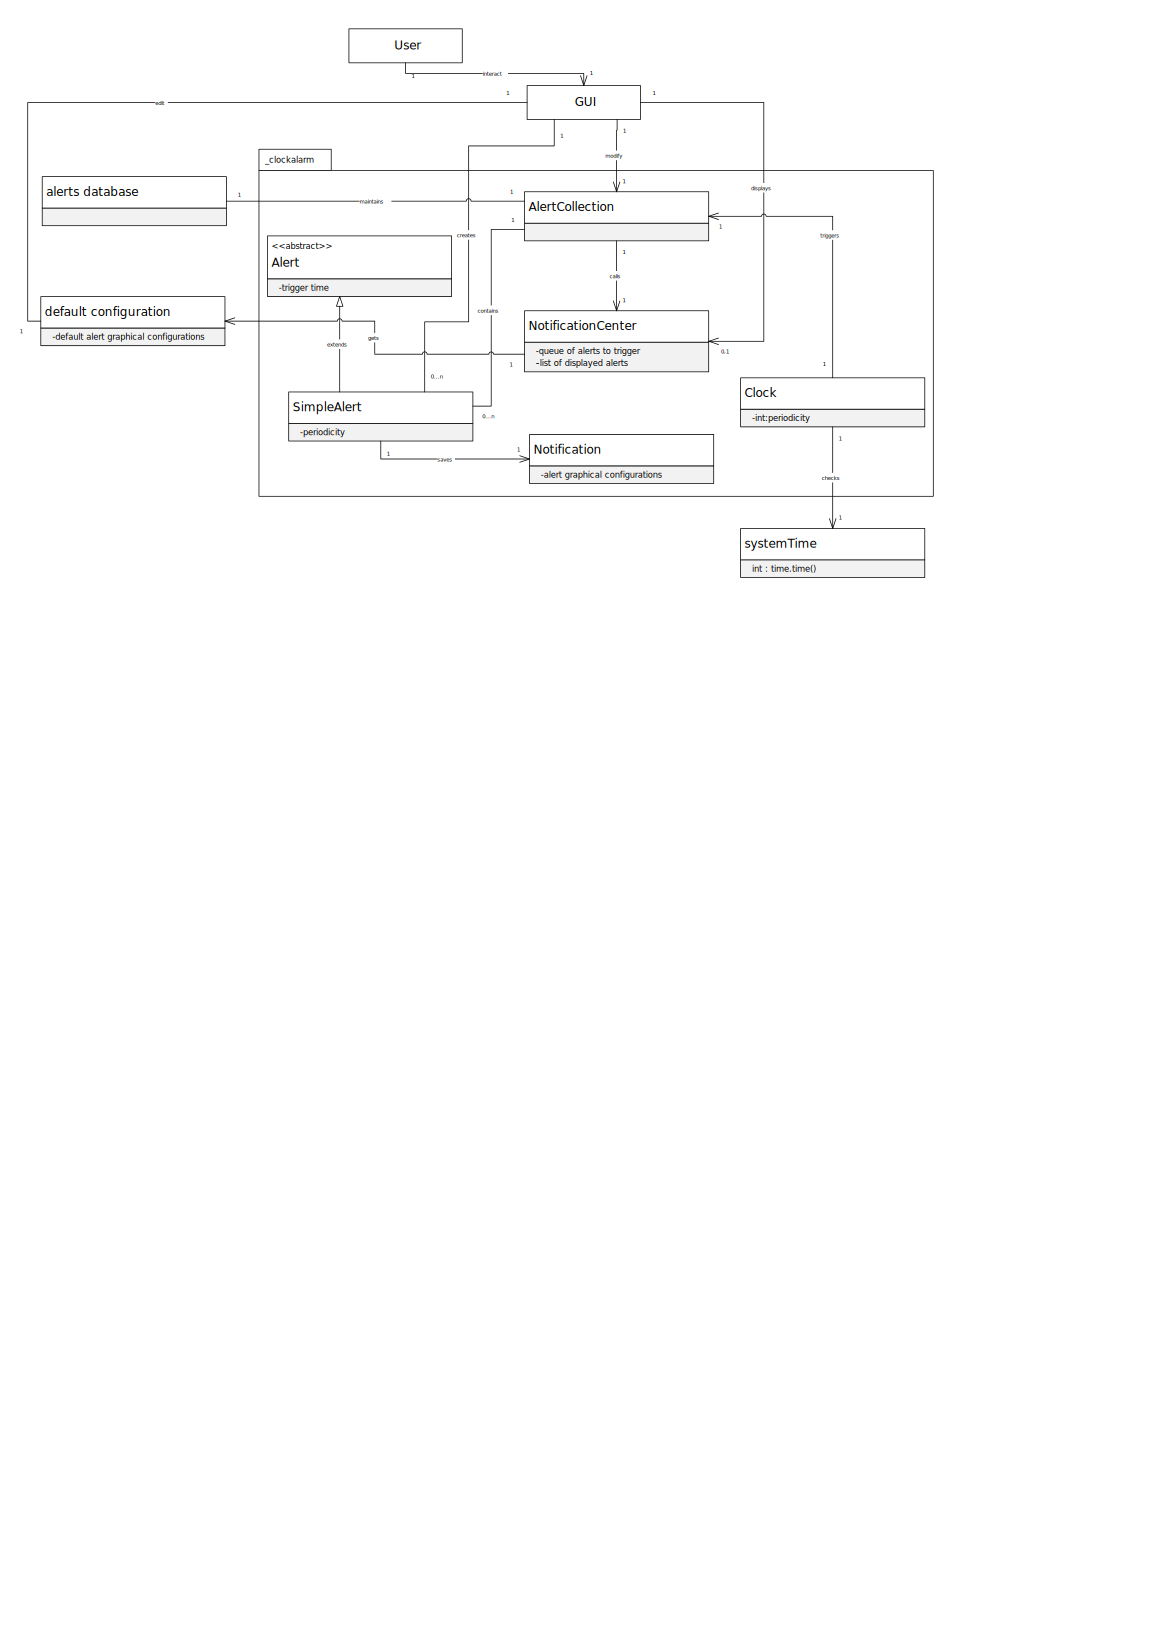
\includegraphics[width=1.0\textwidth]{domain_model.png}
\end{figure}

\section{Use Cases}

All the Use Cases can be found under Appendix \autoref{chap:use_cases}.

\section{Priorities and planning}\label{sec:prio_and_planning}
Description of the various stages of development of the clock alarm product. The versions correspond to the fixed milestones. For each element, a priority is associated.

\begin{tabular}{| r | l | l | l |}
	\hline
	0.2.0 & Time System and Notifications & MH & The program is able to display a hard coded alert, based on the operating system time. \\ \hline
	0.2.1 & \fullref{subsec:usecase_launch} & P2 & The scheduled alert is visible in a GUI before it occures. \\ \hline
	0.3.0 & \fullref{subsec:???} & ? & ? \\ \hline
	0.3.1 & \fullref{subsec:???} & ? & ? \\ \hline
	0.4.0 & \fullref{subsec:???} & ? & ? \\ \hline
	0.4.1 & \fullref{subsec:???} & ? & ? \\ \hline
	0.4.2 & \fullref{subsec:???} & ? & ? \\ \hline
	0.4.3 & \fullref{subsec:???} & ? & ? \\ \hline
	0.4.4 & \fullref{subsec:???} & ? & ? \\ \hline
	0.4.5 & \fullref{subsec:???} & ? & ? \\ \hline
	0.4.6 & \fullref{subsec:???} & ? & ? \\ \hline
	0.4.7 & \fullref{subsec:???} & ? & ? \\ \hline
	0.5.0 & \fullref{subsec:???} & ? & ? \\ \hline
	0.5.1 & \fullref{subsec:???} & ? & ? \\ \hline
	0.2.2 & \fullref{subsec:???} & ? & ? \\ \hline
	0.2.3 & \fullref{subsec:???} & ? & ? \\ \hline
	0.2.1 & \fullref{subsec:???} & ? & ? \\ \hline
	0.2.1 & \fullref{subsec:???} & ? & ? \\ \hline
	0.2.1 & \fullref{subsec:???} & ? & ? \\ \hline
	0.2.1 & \fullref{subsec:???} & ? & ? \\ \hline
	0.2.1 & \fullref{subsec:???} & ? & ? \\ \hline
	0.2.1 & \fullref{subsec:???} & ? & ? \\ \hline
	0.2.1 & \fullref{subsec:???} & ? & ? \\ \hline
	0.2.1 & \fullref{subsec:???} & ? & ? \\ \hline
	0.2.1 & \fullref{subsec:???} & ? & ? \\ \hline
	0.2.1 & \fullref{subsec:???} & ? & ? \\ \hline
	0.2.1 & \fullref{subsec:???} & ? & ? \\ \hline
	0.2.1 & \fullref{subsec:???} & ? & ? \\ \hline
	\hline
\end{tabular}
\section{Gantt Chart}

Please visit
\url{https://bfh-bti7301-project1.github.io/ClockAlarm/gantt/Overview.html} to
get the full Gantt chart of the project.

\section{Technical Requirements}
\label{sec:tech_req}

The priorities are the same as in~\ref{sec:prio_and_planning}, i.e., Must Have
(MH), First Priority (P1), Second Priority (P2), Nice To Have (NTH).

\begin{longtabu}{cccX}
\caption{Technical Requirements Table}
\label{tabu:tech_req}\\

    \toprule
    \taburowcolors~{beaublue..beaublue}
    \textbf{ID}  & \textbf{Status} & \textbf{Prio}  & \textbf{Description}\\
    \taburowcolors~{white..white}
    \toprule
    \endfirsthead\\

    \toprule
    \taburowcolors~{beaublue..beaublue}
    \textbf{ID}  & \textbf{Status} & \textbf{Prio}  & \textbf{Description}\\
    \taburowcolors~{white..white}
    \toprule
    \endhead\\
    
    \taburowcolors~{white..white}
    \multicolumn{4}{r}{\textit{Continued on next page}}\\
    \endfoot
    \bottomrule
    \endlastfoot


    \taburowcolors~{aliceblue..white}
    T.1 & Waiting  & MH & The application shall be written using the python
                          programming language version 3 or greater.\\\midrule
    T.2 & Waiting  & MH & The application shall run on Windows, Linux and
                          macOS.\\\midrule
    T.3 & Waiting  & MH & The database shall be stored in a non binary format.
                          \\\midrule
    T.4 & Waiting  & MH & The application shall still be running after a system
    reboot.\\\midrule
    T.5 & Waiting  & MH & The configuration file shall be OS independent.\\
    \taburowcolors~{white..white}

\end{longtabu}


\section{Quality Requirements}

The priorities are again the same as in~\ref{sec:prio_and_planning}
and~\ref{sec:tech_req}.

\tabulinesep = 1mm
\begin{longtabu}{lccX}
\caption{Quality Requirements Table}
\label{tabu:qual_req}\\
    
    %\toprule
    \taburowcolors~{beaublue..beaublue}
    \textbf{ID}  & \textbf{Status} & \textbf{Prio}  & \textbf{Description}\\
    \taburowcolors~{white..white}
    %\midrule
    \endfirsthead\\

    \multicolumn{4}{c}{\tablename\ \thetable\ --- \textit{Continued from
    previous page}} \\

    %\toprule
    \taburowcolors~{beaublue..beaublue}
    \textbf{ID}  & \textbf{Status} & \textbf{Prio}  & \textbf{Description}\\
    \taburowcolors~{white..white}
    %\midrule
    \endhead\\
    
    \taburowcolors~{white..white}
    \multicolumn{4}{r}{\textit{Continued on next page}}\\
    \endfoot
    %\bottomrule
    \endlastfoot

    \taburowcolors~{aliceblue..white}
    Q.1 & Done & MH & The application shall display an alert on the screen
    within a second at the specified date and time of the alert.\\%\midrule
    \taburowcolors~{white..white}
    Q.2     & Partially Done & P1 & User Interface.\\
    Q.2.1   & Done  & P1 & The main user interface shall contain buttons to
    create, edit, delete alerts.\\
    Q.2.2   & Not done & P1 & The main user interface shall contain buttons to
    create, edit, delete categories.\\
    Q.2.3   & Done  & P1 & The main user interface shall contain a button to
    access the preferences.\\
    Q.2.4   & Done  & P1 & The main user interface shall contain a button to
    snooze the alerts appearing on the screen.\\
    Q.2.5   & Done  & P1 & The main user interface shall contain an area
    where all the alerts are listed.\\
    Q.2.6   & Partially Done & P2 & The user shall be able to sort the alerts by
    category, by due date and alphabetically.\\

    \taburowcolors~{white..white}

\end{longtabu}


\chapter{Diagrams}

\section{Class Diagrams}
\subsection{Simple alerte Notification}
Used for the Milestone ``Version 0.2.0 - Time system and notification''.

\begin{figure}[h]
	\centering
	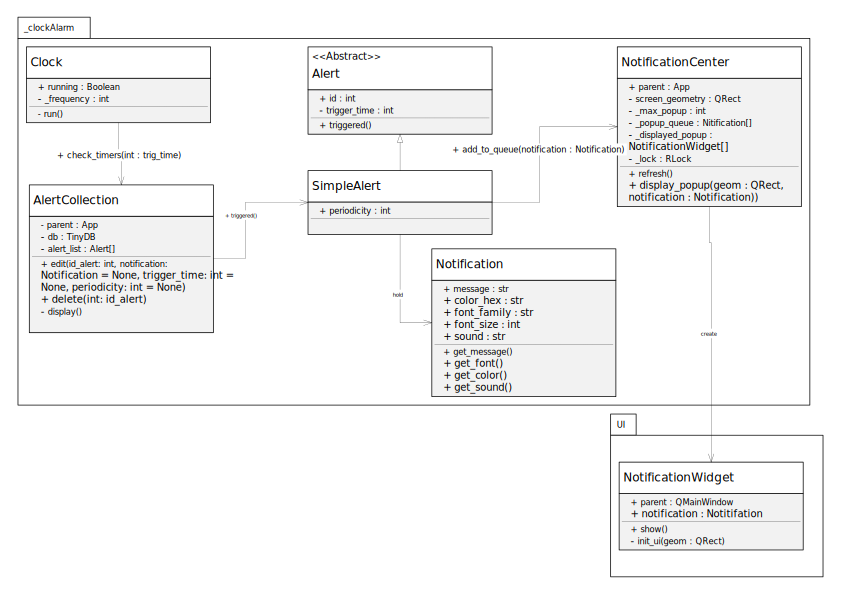
\includegraphics[width=1.0\textwidth]{class_diagram_simple_alert_notification.png}
\end{figure}

\section{Sequence Diagrams}
\subsection{Simple alerte Notification}
Used for the Milestone ``Version 0.2.0 - Time system and notification''.

\begin{figure}[h]
	\centering
	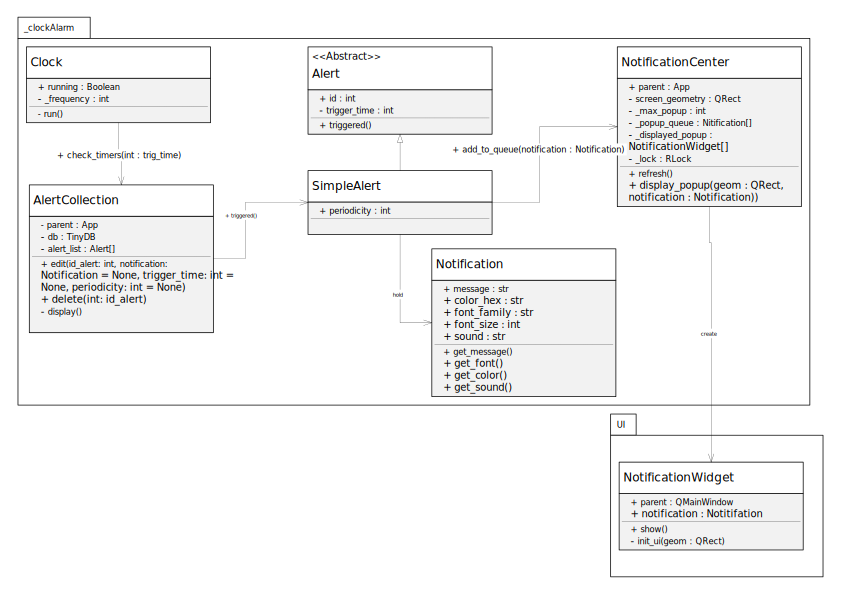
\includegraphics[width=1.0\textwidth]{class_diagram_simple_alert_notification.png}
\end{figure}
\chapter{Development decisions}

The structure of the development process of this project is based on the book
`Requirements Engineering Fundamentals`\cite{pohl2011requirements}.

\subsection{Word Processor}
In order to write this document, we had to choose between several word processors. We required that the file could be used with a version control system so that the documentation and code could live in the same place. Also we didn't want to loose time if there was a need to change the layout. After discussion, we came up with the following list:
\begin{enumerate}
\item \Gls{microsoft_word}
\item \Gls{google_docs}
\item \Gls{libre_office}
\item \Gls{scribus}
\item \Gls{tex}
\end{enumerate}
The main problem with number 1 and 3 is that the output of these programs are binary files. A built in versioning functionality exits in \gls{microsoft_word} but it adds another version control layer to the workflow. The .docx and .odt file types are in fact ZIP archives containing XML documents which can be uncompressed. They could be stored in the uncompressed state to be compatible with the chosen version control system. Or they could be converted into another format. Clearly this is not convenient. Therefore we decided that they were not compatible with our first requirement stated above.\\
Using a Google Doc means that the document will be stored on Google's servers and not within the folder containing the source code. I thus also violates our first requirement.\\
%\Gls{scribus} is a free alternative to \gls{indesign}. It doesn't produce binary files
\chapter{Version Control}\label{ch:version}

\tabulinesep = 1mm
\begin{longtabu}{lccX}
\caption{Version Control Table}
\label{tabu:tech_req}\\
    %\toprule
    \taburowcolors~{beaublue..beaublue}
    \textbf{Version}  & \textbf{Date} & \textbf{Description}  & \textbf{Author}\\
    \taburowcolors~{white..white}
    %\midrule
    \endfirsthead\\
    %\toprule
    \taburowcolors~{beaublue..beaublue}
    \textbf{Version}  & \textbf{Date} & \textbf{Description}  & \textbf{Author}\\
    \taburowcolors~{white..white}
    %\midrule
    \endhead\\
    
    \taburowcolors~{white..white}
    \textbf{Version}  & \textbf{Date} & \textbf{Description}  & \textbf{Author}\\
    \endfoot
    %\bottomrule
    \endlastfoot
    \taburowcolors~{aliceblue..white}
    X0.1 & 26.02.2017 & Initialization of the requierments document  & Samuel Gauthier\\%\midrule
    X0.2 & 13.03.2017  & Update of the requierments documentation & Loïc Charrière\\%\midrule
    X1.0 & 28.05.2017  & Document ready for review & Samuel Gauthier\\%\midrule
    V1.0 & 29.05.2017  & Document ready for handout & Loïc Charrière\\
    V1.4 & 10.06.2017  & Document revision & Samuel Gauthier\\
    \taburowcolors~{white..white}
\end{longtabu}

\section{Python}
<<<<<<< HEAD
As two teams separately developed a similar \gls{kalarm} project, the decision was made to realize our project in python.

\gls{python} is a relatively old programming language, as it appeared in 1991. This makes the \gls{python}'s libraries extremely numerous and diversified. However, many of them are no longer updated. \gls{python} has a simple easy to learn syntax. It is object-oriented and cross-platform. It was mainly disigned for prototyping, which means that it is possible to obtain a functional and efficient code in a minimum amound of time.

=======
As two teams separately developed a similar \gls{kalarm} project, the decision was made to realize our project in python.\\
\gls{python} is a relatively old programming language, as it appeared in 1991. This makes the \gls{python}'s libraries extremely numerous and diversified. However, many of them are no longer updated. \gls{python} has a simple easy to learn syntax. It is object-oriented and cross-platform. It was mainly disigned for prototyping, which means that it is possible to obtain a functional and efficient code in a minimum amound of time.\\
>>>>>>> d7fbb24d58d8a58d2f9522ce928d452beb7433d2
\gls{python}'s detractors reproach it his lack of security mechanisms compared with traditional languages. Indeed, \gls{python} follows the philosophy of Linux, which count on a solid OS capable of protecting the code it uses, not a code that protects itself.
\section{Unit Testing}

Python comes with a couple of built-in modules for testing the source code:

\begin{enumerate}
    \item Unittest
    \item Doctest
    \item Unittest.mock (Only for Python 3.3)
\end{enumerate}

The Unittest framework is similar to the JUnit one: ``It supports test
automation, sharing of setup and shutdown code for tests, aggregation of tests
into collections, and independence of the tests from the reporting
framework.''~\cite{pythondoc361unittest}

Doctests are put in comments and are formatted in form of an interactive Python
session. They are usually very simple and give informative examples of the usage
of the class or function to the reader.~\cite{python361doctest}

Unittest.mock allows to replace parts of the system under test with mock objects
and make assertions about how they have been used.~\cite{pythondoc370mock}
\\

Other alternatives include: pytest, nose2 and tox.

Pytest makes it easy to write tests: only plain assert statements are used,
which makes the code look very clean and neat. It can run unittest and nose test
suites without any additional configuration nor modification.~\cite{pytest}

Nose2 is the successor of nose. Its goals are to extend unittest and make
testing easier to understand.~\cite{nose2VSnose}

Tox is a test framework and virtualenv management tool that allows to run tests
in multiple environments.~\cite{tox270doc}\\

We chose to use pytest because as already mentioned, the code is cleaner and
more readable. Less work is also required to achieve the same result as with the
other solutions. We do not use virtual environments so tox is of no use to us.

\section{Code Coverage}

There is at the moment only one maintained mature tool for measuring the code
coverage in Python: Coverage.py.\footnote{Nose provides code coverage but it is
deprecated and being replaced by nose2, still under development.} ``It monitors
your program, noting which parts of the code have been executed, then analyzes
the source to identify code that could have been executed but was
not.''\cite{coveragePY} It also provides clean and readable annotated html
reports.

\section{Documentation}\label{sec:documentation}

For documenting our project we use Sphinx%
\footnote{\url{http://www.sphinx-doc.org}} combined with Read
The Docs\footnote{\url{https://readthedocs.org}} to host the
documentation. Read The Docs builds the documentation every time there is a new
commit (A git hook has to be set up beforehand for it to work).

We choose Sphinx because it is the most popular tool used in the python
community and it is officially recommended (The official Python documentation is
created using Sphinx).

During development we realised thanks to Sphinx that our project had cycles. See
Section~\ref{sec:cycles} for additional details.

After retrospection, this document could have been written using Sphinx. It has
the same capabilities than \LaTeX{} and can generate the document in multiple
formats: pdf, html, etc..

\section{System Notifications}

We first tried to use the OS specific system notification API.\@With this
solution we didn't have to care were the notifications would appear on the
screen. They would always be at the correct position on every platform. There is
however one drawback: the notifications cannot be fully customized. Only the
icon can be changed but the typeface and the sound cannot. This is why we choose
to develop our own notification system, \texttt{Notification.py}, where
notifications can be fully customized.

\section{GUI}

As our application has to run on multiple platforms, the GUI framework should
also support multiple platforms. The framework should also support Python 3. The
Python wiki lists over 35 frameworks, many of those target \gls{qt}. We have chosen
only three that were recommended by the
\citetitle{schlusser2016hitchhikers}~\cite{schlusser2016hitchhikers}:

\begin{enumerate}
    \item PySide
    \item PyQt
    \item Tk
\end{enumerate}

PySide, as PyQt, provides a binding to the \gls{qt} framework. The main difference
between the two is the license: PySide uses the \acrfull{lgpl} whereas PyQt uses
the \acrfull{gpl}. Which means that source code licensed under the
\acrshort{gpl} must be opensource. On the other hand the
\acrshort{lgpl} is more suited for closed source projects. In addition PyQt
supports Python 3. Tk provides bindings to the Tk framework and is licensed
under a \acrfull{bsd} license.

We chose the PyQt framework out of personal preference. All three frameworks
are equally well suited for a project like this one.




\section{Database}

We planned to have three alert types:

\begin{enumerate}
    \item Simple non recurring text alerts
    \item Recurring simple alerts
    \item Alerts that send emails
\end{enumerate}

All three types are independent of each other, that is, there is no logical link
between them. The only ``link'' that they have in common is that they are
extending the abstract class \texttt{Alert}. Therefore we don't need a
relational database, only a very lightweight one.

The requirement for the file storing the database is that it should be humanly
readable, i.e., it should be in a non binary format. We came up with four
possibilities for the file format:

\begin{itemize}
    \item XML
    \item JSON
    \item YAML
    \item Plaintext
\end{itemize}

BaseX\footnote{For python it is the BaseXCLient:
\url{http://basex.org}} handles both JSON and XML databases. Another
alternative is TinyDB
\footnote{\url{http://tinydb.readthedocs.io}}, it
handles only databases in the JSON format. PyXAML
\footnote{\url{http://pyyaml.org}} handles databases stored in the
YAML
format. And for a plaintext database, i.e., a simple text file, everything has
to be handled with the Python \texttt{open(\ldots)} and \texttt{write(\ldots)}
commands.

We choose to use TinyDB and the JSON file format because our supervisor
encouraged us to do so and because the syntax is very simple and follows the
Pythonic way.


\chapter{Minutes}
\section{Meeting~\arabic{section}: March 1, 2017}
\subsection*{Present at meeting}
Samuel Gauthier, Loïc Charrière, Claude Fuhrer
\subsection*{Agenda}
\begin{itemize}
	\item Present  the Use Cases  and User stories
	\item Discussion about the usage of Python
\end{itemize}
\subsection*{Notes}
	\subsubsection{Use Cases and User stories}
	\begin{itemize}
        	\item Vision\&Goals: The vision and goals of the project have to be enhanced and not taken ``as is''.
		\item If a choice is made during the project, we should write down why it has been made this way. Everything that hasn't been documented is considered not been done.
		\item If we go for a specific product (such as DBMS, module, etc.) we should at least try out other alternatives (2--3) and explain why we made the choice of using this specific product.
		\item Split the user story ``reate/delete categories'' in two.
		\item Sort the uses cases by topic.
		\item Alarms could be snoozed. (for example, if the user is at a meeting snooze all alarms so that they don't disturb the meeting) 
		\item Alarms should be user specific, i.e., they should belong to the user connected on the computer and not be shared across all the users of the machine.
		\item Book recommendation (chapter about use cases) -> Applying UML and Patterns (Larman).
	\end{itemize}
	\subsubsection{Usage of Python}
	\begin{itemize}
		\item Strongly discouraged to share python code via e-mail (General life advice)
		\item Code coverage 70--80\% is ok, 30\% is not
        \end{itemize}
\subsection*{Tasks}
	\begin{itemize}
		\item Improve vision\&goals
		\item Create use cases / user stories / actors correctly
		\item Read Python doc
	\end{itemize}
\subsection*{Next Meeting}
\st{TBD} (edit)
March 17, 2017

\section{Meeting~\arabic{section}: March 17, 2017}
\subsection*{Present at meeting}
Samuel Gauthier, Loïc Charrière, Claude Fuhrer
\subsection*{Agenda}
\begin{itemize}
    \item System and Context Boundaries
    \item System diagrams
    \item System description
\end{itemize}
\subsection*{Notes}
    The Project Goals should not be written down as a list. We need to create
    full sentences in order to help the reader's comprehension.\\
    \textbf{Question:} ``Should this document contain snippets of code?''\\
    \textbf{Answer:} It depends on the target audience. But here we should
    only show snippets of pseudo code for complicated parts of our code.
    \subsubsection{System and Context Boundaries}
    \begin{itemize}
        \item Some of the Stakeholders will not influence our project. They
            are only there so that our documentation is complete.
    \end{itemize}
    \subsubsection*{System diagrams}
    \begin{itemize}
        \item Good domain model.
        \item The domain model should contain types only if they
            are very specific and part of the DM\@.
        \item It is not useful to specify interfaces and abstract classes.
    \end{itemize}
    \subsubsection*{System description}
    \begin{itemize}
        \item We need to link the User Stories and Use Cases.
    \end{itemize}
    \subsection*{Other}
    \textbf{Question:} ``How should our workflow be? Should we write the
    documentation and the code at the same time?''\\
    \textbf{Answer:} We shouldn't waste too much time on writing documentation.
    Basically we should use the Scrum method. All the Use Cases (or the most
    important ones) have to be written down. Then we can decide what has to
    be included in each sprints. For each sprint we must have a working version
    of our application. Start with a small version having the alerts date
    hard coded in the code, with no GUI.\@ Then add a new feature with each
    sprints.
\subsection*{Tasks}
    \begin{itemize}
        \item Rewrite the Project Goals
        \item Prepare sprints
    \end{itemize}
\subsection*{Next Meeting}
TBD

\section{Meeting~\arabic{section}: April 7, 2017}

\subsection*{Present at meeting}
Samuel Gauthier, Loïc Charrière, Claude Fuhrer

\subsection*{Agenda}
\begin{itemize}
    \item Show version with a simple notification
\end{itemize}

\subsection*{Notes}

The \texttt{setup.py} is useful for bigger projects but in our case it
is not. If we have time at the end then we should implement it.

The autostart function should be cared of only at the very end of the
project.  Users can do it themselves at the moment. More important are the
persistence and customization features.

\textbf{Question:} Should we create one thread for every alarm or one
thread for the hole program?

\textbf{Answer:} The best solution is to create one thread for the hole
program that checks the due time ever 30 seconds or every minute.

Logging is useful and should be preferred instead of simple prints
because it is possible to disable it completely for a project.

\subsection*{Tasks}
    \begin{itemize}
        \item Document Use Case ``Notification Center''.
        \item Write the encountered development problems in the documentation.
    \end{itemize}
\subsection*{Next Meeting}
TBD



\printglossaries{}

\printbibliography[
heading=bibintoc,
title={Bibliography}
]

\end{document} 
